\documentclass[a4paper,10pt]{article}
\usepackage{geometry}
\usepackage{xeCJK}
\usepackage{fancyhdr}  % 页眉页脚
\usepackage{minted}    % 代码高亮
\usepackage{pdfpages}
%\usepackage[colorlinks]{hyperref}  % 目录可跳转
\usepackage[pdfstartview=FitH,
CJKbookmarks=true,
bookmarksnumbered=true,
bookmarksopen=true,
colorlinks,
pdfborder=001,
linkcolor=blue,
anchorcolor=blue,
citecolor=blue,
]{hyperref}
\usepackage{tikz} %加水印用
\usepackage{eso-pic}
\usepackage{lastpage}
\usepackage{bookmark}
\usepackage{titletoc}


\hypersetup{hidelinks}

\setlength{\headheight}{15pt}
\contentsmargin{0pt}\renewcommand\contentspage{\thecontentspage}
\dottedcontents{section}[2.3em]{}{2.3em}{5pt}
\dottedcontents{subsection}[5.5em]{}{3.2em}{5pt}


\geometry{left = 2.0cm,right=2.0cm,top=2.5cm,bottom=2.5cm}

\newcommand \BackgroundPicture{%
    \put(0,0){%
        \parbox[b][\paperheight]{\paperwidth}{%
            \vfill
            \centering%
            \begin{tikzpicture}[remember picture,overlay]
            \node [rotate=60,scale=20,text opacity=0.1] at (current page.center) {tabris}; %中括号内是旋转角度,字体大小
            \end{tikzpicture}%
            \vfill
}}}


% 定义页眉页脚
\pagestyle{fancy}
\fancyhead{}
\fancyhead[C]{Algorithm Library by tabris} 

\fancyfoot{}                                               
\fancyfoot[C]{- \thepage\ -}
\renewcommand{\headrulewidth}{0.4pt} \renewcommand{\footrulewidth}{0.4pt}


\author{tabris}   
\title{Algorithm Library}



\begin{document} 

    
	\maketitle % 封面
	%\setcounter{page}{1}
    \AddToShipoutPicture{\BackgroundPicture}
	\thispagestyle{empty}
	\newpage % 换页
	\pagenumbering{Roman}
	\tableofcontents % 目录
	\newpage
	\pagenumbering{arabic}
	\part{Graph Theory}
		% 基础
		\section{Basement} % 二级标题
			\subsection{Representation}
				\inputminted[breaklines]{c++}{graph/base.cc} % 插入代码文件
		
		%最短路
		\section{Shortest Path}
			\subsection{SPFA}
				\inputminted[breaklines]{c++}{graph/SPFA.cc}
			\subsection{Dijkstra}
				\inputminted[breaklines]{c++}{graph/dijkstra.cc}
				
		%最小生成树
		\section{Minimum Spanning Tree}
			\subsection{Kruskal}
				\inputminted[breaklines]{c++}{graph/kruskal.cc}
			\subsection{Prim}
				\inputminted[breaklines]{c++}{graph/Prim.cc}
				
		% 有向图
		\newpage
		\section{Directed Graph}
			\subsection{Topological Sorting}
				\inputminted[breaklines]{c++}{graph/Topological-Sorting.cc}
		
		% 二分图
		\newpage
		\section{Bipartite Graph}
			\subsection{Hungary}
				\inputminted[breaklines]{c++}{graph/Bipartite_Graph.cc}
			\subsection{Two Set}
				\inputminted[breaklines]{c++}{graph/Two-set.cc}

		% 强联通
		\newpage
		\section{Strongly Connected}
			\subsection{tarjon}
				\inputminted[breaklines]{c++}{graph/Strongly_Connected.cc}
		
		% 树 : 重心,直径,中心边
		\newpage
		\section{Tree}
			\subsection{centre of gravity of tree}
				\inputminted[breaklines]{c++}{graph/centre_of_gravity_of_tree.cc}
             \newpage
			\subsection{Least Common Ancestors}
				\inputminted[breaklines]{c++}{graph/lca.cc}
		\section{Network Flows}
			\subsection{Dinic}
				\inputminted[breaklines]{c++}{graph/dinic.cc}
            \subsection{ISAP}
                \inputminted[breaklines]{c++}{graph/isap.cc}
	
	%\twocolumn  % 分页显示
	\newpage
	\part{String}
		\section{String Match}
			\subsection{KMP}
				\inputminted[breaklines]{c++}{String/kmp.cc}
		
			\subsection{Trie}
				\inputminted[breaklines]{c++}{String/Trie.cc}
			
			\subsection{Aho Corasick Auto Mation}
				\inputminted[breaklines]{c++}{String/Aho-Corasick_Auto_Mation.cc}
			
			\subsection{Suffix Arrays}
				\inputminted[breaklines]{c++}{String/Suffix_Arrays.cc}
			\newpage
			\subsection{Suffix Automaton}
				\inputminted[breaklines]{c++}{String/suffix-automaton.cc}
				
		\newpage
		\section{Manachar}
			\inputminted[breaklines]{c++}{String/Manachar.cc}
	
	
	\newpage
	\part{Data structure}
		\section{UFS}
			\inputminted[breaklines]{c++}{Date_structure/UFS.cc}
			
		\section{BIT}
			\inputminted[breaklines]{c++}{Date_structure/BIT.cc}
			
		\section{Segment tree}
			\inputminted[breaklines]{c++}{Date_structure/Segment_tree.cc}
			
		\section{Chair tree}
			\inputminted[breaklines]{c++}{Date_structure/Chair_tree.cc}
			
		\section{Splay}
			\inputminted[breaklines]{c++}{Date_structure/Splay.cc}
           
		\section{Link Cut Tree}
            \inputminted[breaklines]{c++}{Date_structure/lct.cc}
        \newpage
		\section{KD-tree}
			\inputminted[breaklines]{c++}{Date_structure/KD-tree.cc}
			
		\section{tranform : tree -> arrary}
			\subsection{dfs order}
				\inputminted[breaklines]{c++}{Date_structure/dfs_order.cc}
			\subsection{Heavy light Decomposition}
				\inputminted[breaklines]{c++}{Date_structure/Heavy_light_Decomposition.cc}
		\section{SparseTable}
			\inputminted[breaklines]{c++}{Date_structure/SparseTable.cc}
    
    	\section{Leftist Tree}
              \inputminted[breaklines]{c++}{Date_structure/Leftist-Tree.cc}
	\newpage
	\part{Math} % 一级标题
		\section{Number Theory}
			\subsection{Basement}
			
	            \textbf{费马小定理}  :  $a^{p-1} \equiv 1 \pmod p$\\
				\textbf{欧拉定理}    :  $a^{\varphi(m)} \equiv 1 \pmod m$ $\varphi()$为欧拉函数\\
				\textbf{殴拉降幂}    :  $A^x\%C=A^{x\%\varphi(C)+\varphi(C)}\%C,(x\ge \varphi(C))$\\
				\textbf{威尔逊定理}  :  $(p-1)!\equiv -1 \pmod p$\\
				\textbf{素数距离}    :  任意两个相邻素数距离不超过 $246$ (截止$2014$年$2$月)\\
				\textbf{唯一分解定理}:  对于任意一个$N$我们可以写成$N=P_1^{a_1}*P_2^{a_2}*P_3^{a_3}*...*P_n^{a_n}$
				
				\subsubsection{inverse}
					\inputminted[breaklines]{c++}{Math/inverse.cc}
                \subsubsection{Guass}
                    \inputminted[breaklines]{c++}{Math/Guass.cc}
                \subsubsection{linear basis}
                    \inputminted[breaklines]{c++}{Math/linear-basis.cc}
                    
			\subsection{Congruence problem}
                余数定理:\\
                \\
                计算$\left(\frac{a}{b}\right)\pmod{c}$ ,其中$b$能整除$a$\\
                如果$b$与$c$互素,则$(\frac{a}{b})\%c=a*b^{phi(c)-1}\%c$\\
                如果$b$与$c$不互素,则$(\frac{a}{b})\%c=\frac{a\%(b*c)}{b}$\\
                对于$b$与$c$互素和不互素都有$(\frac{a}{b})\%c=\frac{a\%(b*c)}{b}$成立\\
                \subsubsection{gcd}
                    \inputminted[breaklines]{c++}{Math/exgcd.cc}
                \subsubsection{China remainder theory}
                    \inputminted[breaklines]{c++}{Math/CRT.cc}
                \subsubsection{Function Of Congruence}
                    \inputminted[breaklines]{c++}{Math/function-of-Congruence.cc}
                    
			\subsection{Prime}
                \subsubsection{Sieve}
                    \inputminted[breaklines]{c++}{Math/sieve.cc}
                \subsubsection{Fundamental Theorem of Arithmetic}
                    \inputminted[breaklines]{c++}{Math/Fundamental-Theorem-of-Arithmetic.cc}
				\subsubsection{Miller Rabbin}
					\inputminted[breaklines]{c++}{Math/miller-rabbin.cc}
				\subsubsection{Pollard Rho}
					\inputminted[breaklines]{c++}{Math/pollard_rho.cc}
                \subsubsection{count primes}
                    \inputminted[breaklines]{c++}{Math/Meissel-Lehmer.cc}
					
			\subsection{Multiplicative Function}
				\subsubsection{Euler Function}
					欧拉函数 $\varphi(n)$\\
					
					$\varphi(n)$积性函数,对于一个质数$p$和正整数$k$,有\\ 
					$\varphi(p^k) = p^k - p^{k-1} = (p - 1)p^{k - 1} = p^k(1 - \frac{1}{p})$\\
					
					$n = \sum_{d|n}\varphi(d)$\\
					当$n > 1$时,$1 … n$中与n互质的整数和为$n$$\frac{\varphi(n)}{2}$\\
					\inputminted[breaklines]{c++}{Math/Euler.cc}
			
			\subsection{Fast Calculation}
				\subsubsection{Fast Exponentiation Mod}
					\inputminted[breaklines]{c++}{Math/Fast-Exponentiation-Mod.cc}
				\subsubsection{Fast Multi}
					\inputminted[breaklines]{c++}{Math/Fast-Multi.cc}
				\subsubsection{Fast Sqrt}
					\inputminted[breaklines]{c++}{Math/Fast-Sqrt.cc}
				\subsubsection{Matrix}
					\inputminted[breaklines]{c++}{Math/Matrix.cc}
				\subsubsection{Fast Fourier Transform}
					\inputminted[breaklines]{c++}{Math/FFT.cc}
				\subsubsection{Fast Number Theoretic Transform}
					\inputminted[breaklines]{c++}{Math/NTT.cc}
				\subsubsection{Fast Walsh Transform}
					\inputminted[breaklines]{c++}{Math/FWT.cc}
            \subsection{Primitive Root}
                \textbf{原根}\\
                \textbf{定义}:设$m>1$,$\gcd(a,m)=1$,使得$a^{r} \equiv \pmod {m}$成立的最小的$r$,称为$a$对模$m$的阶,记为.$\delta_{m}(a)$\\
                
                \textbf{定理}:如果模$m$有原根,那么它一共有个$\varphi(\varphi(m))$原根.\\
                
                \textbf{定理}:若$m>1$,$\gcd(a,m)=1$,$a^{n} \equiv\pmod {m}$则$\delta_{m}(a)|n$.\\
                
                \textbf{定理}:如果$p$为素数,那么素数$p$一定存在原根,并且模$p$的原根的个数为$\varphi(p-1)$.\\
                
                \textbf{定理}:设$m$是正整数,$a$是整数,若$a$模$m$的阶等于$\varphi(m)$,则称$a$为模$m$的一个原根.\\
                
                假设一个数$g$对于模$m$来说是原根,那么$g^{i}\pmod {p}$的结果两两不同,且有$1< g< p$,$0\leq i< p$那么$g$可以称为是模$p$的一个原根,归根到底就是$g^{p-1}\equiv \pmod {p}$当且仅当指数为$p-1$的时候成立.(这里是素数)\\
                
                模$m$有原根的充要条件:$m=2,4,p^a,2p^a$,其中$p$是奇素数.\\
                
                
                求模素数$P$原根的方法:对$p-1$素因子分解,即$p-1=p_1^{a_1}p_2^{a_2}...p_k^{a_k}$是的标准分解式,若恒有
                $g^{\frac{p-1}{p_i}} \neq 1\pmod {p}$成立,则$g$就是$p$的原根.(对于合数求原根,只需把$p-1$换成$\varphi(p)$即可)\\
                \inputminted[breaklines]{c++}{Math/Primitive-Root.cc}
				
		\section{Combinatorial mathematics}
			\subsection{combinatorial number}
                \subsubsection{M个盘子取N个球}
                    1: 球同,盒同,盒不可以为空   $P_m(N)$-这符号表示部分数为$m$的$N$-分拆的个数. \\
                    2: 球同,盒同,盒可以为空     $P_m(N+M)$ 为什么要加$M$,与$4$为什么要在$3$的基础上加$M$是一样的,就是为了保证不为空        \\
                    3: 球同,盒不同,盒不可以为空 $C(N-1, M-1)$ \\
                    4: 球同,盒不同,盒可以为空   $C(N+M-1, M-1)$ \\
                    5: 球不同,盒同,盒不可以为空 $S(N, M)$ --第二类斯特林数\\
                    6: 球不同,盒同,盒可以为空   $S(N,1) + S(N, 2) + S(N, 3) + ... + S(N, M)$\\
                    7: 球不同,盒不同,盒不可以为空 $ M! * S(N, M)$\\
                    8: 球不同,盒不同,盒可以为空 $M^N$  --表示$M$的$N$次方\\
				\subsubsection{Pascal's Triangle}
					\inputminted[breaklines]{c++}{Math/Pascal-Triangle.cc}
				\subsubsection{factorial/inverse}
					\inputminted[breaklines]{c++}{Math/C(n,m).cc}
				\subsubsection{Lucas}
					\inputminted[breaklines]{c++}{Math/lucas.cc}
			
			\subsection{Catalan number}
				\inputminted[breaklines]{c++}{Math/Catalan.cc}
			\subsection{Stirling number[one]}
				\inputminted[breaklines]{c++}{Math/Stirling-number-one.cc}
			\subsection{Stirling number[two]}
				\inputminted[breaklines]{c++}{Math/Stirling-number-two.cc}
			\subsection{Bell number}
				\inputminted[breaklines]{c++}{Math/Bell.cc}
			\subsection{Principle of inclusion-exclusion} %容斥原理
				\inputminted[breaklines]{c++}{Math/rongchi.cc}
			\subsection{Möbius inversion formula} %莫比乌斯反演
				
					设$f$为算术函数,$f$的和函数$F$为$F(n)=\sum_{d|n}f(d)$,它是依据$f$的值决定的.是否存在一种用$F$求$f$的简单方法?这就是\textbf{莫比乌斯反演公式}\\
					
					莫比乌斯函数\\
					
					$ \mu(n) = \left\{\begin{array}{rcl} 1 && ,n=1\\ (-1)^r && ,n=p_1*p_2*...*p_r \\0 && ,other \end{array}\right.$\\
					
					莫比乌斯函数是一个\textbf{乘性函数}\\
					
					莫比乌斯函数的和函数$F$,$F(n) = \sum_{d|n} \mu (d)$ 满足
					$ F(n) = \sum_{d|n}\mu(d) = \left\{\begin{array}{rcl} 1 && ,n=1  \\0 && ,n>1 \end{array}\right.$
					
					\textbf{莫比乌斯反演公式}\\
					对于$f$与其和函数$F(n)=\sum_{d|n}f(d)$\\
					形式一:$f(n) = \sum_{d|n}\mu(d)F(\frac{n}{d})$\\
					形式二:$f(n) = \sum_{n|d}\mu(\frac{d}{n})F(d)$
					
					注意有这样的两种形式,
				
				\inputminted[breaklines]{c++}{Math/mobius.cc}
        
		\newpage
		\section{Game Theory}
			\subsection{Wythoff Game}
				\inputminted[breaklines]{c++}{Math/Wythoff.cc}
			\subsubsection{Sprague Grundy}
                \inputminted[breaklines]{c++}{Math/SG.cc}
	
	% 计算几何
	\newpage
	\part{Computational Geometry}
        \section{向量旋转}
        我们想将向量 $\overrightarrow {x, y}$ 以$x$为轴点逆时针旋转,且旋转角为 $\alpha $\\ \\
        $ \left[\begin{array}{cc}\  x' \\   y' \end{array}\right]=\left[\begin{array}{cc}\ \cos(\alpha) &-\sin(\alpha) \\   \sin(\alpha) & \cos(\alpha) \end{array}\right] \times \left[\begin{array}{cc}\  x \\   y \end{array}\right]$
        \section{Various Code}
            \subsection{2-D}
                \inputminted[breaklines]{c++}{ComputationalGeometry/2-d.cc}
            \subsection{3-D}
                \inputminted[breaklines]{c++}{ComputationalGeometry/3-d.cc}
	
	\newpage
	\part{STL} % 一级标题
		\section{Set}
			\inputminted[breaklines]{c++}{STL/set.cc}
		\section{Multiset}
		 	\inputminted[breaklines]{c++}{STL/multiset.cc}
		\section{bitset}
			\inputminted[breaklines]{c++}{STL/bitset.cc}
		\section{Map}
			\inputminted[breaklines]{c++}{STL/map.cc}
        \section{HashMap}
            \inputminted[breaklines]{c++}{STL/Hashmap.cc}
		\section{Queue}
			\inputminted[breaklines]{c++}{STL/queue.cc}
	
	\newpage
	\part{Other} % 一级标题
        \section{Divide}
            \subsection{Normal Divide}
                \textbf{For Example :}\underline{\textbf{marge sort}}\\
                    \inputminted[breaklines]{c++}{Other/normal-divide.cc} 
                
                \textbf{For Example :}\underline{\textbf{平面最近点对}}\\
                \inputminted[breaklines]{c++}{Other/normal-divide-2.cc}
                
            \subsection{Tree Divide}
                \subsubsection{Point Divide}
                    \textbf{For Example :}\\
                    \\
                    Description: 给你一棵树,问你两点间距离不超过k的点对个数\\
                    Solve      : 点分治,每次找重心,求经过重心的满足的解的个数,最后累加.
                    \inputminted[breaklines]{c++}{Other/point-divide.cc}
                \newpage
                \subsubsection{Edge Divide}
                    \textbf{For Example :}\\
                    \\
                    Description: \\
                    给你一棵树,同样是两个操作:\\
                    (1)单点颜色修改\\
                    (2)询问整棵树中,最远的白色两点的距离$<==>$ $max{dist(a,b)},color[a]=color[b]=white$.\\
                    Solve      : 边分治,每次找中心边,求经过中心边的满足的最远距离,最后维护.\\
                    注意面对菊花树的时候边分治会退化,所以要加虚点变成二叉树\\
                    具体也不大会,看命吧\\
                    \inputminted[breaklines]{c++}{Other/edge-divide.cc}
            \newpage
            \subsection{CDQ Divide}
                \inputminted[breaklines]{c++}{Other/cdq-divide.cc}
                  
        \newpage
		\section{手动开栈}
			\inputminted[breaklines]{c++}{Other/stack.cc}
		\section{fastIO}
			\inputminted[breaklines]{c++}{Other/fastio.cc}
		%\section{fread}
		%	\inputminted[breaklines]{c++}{Other/Fread.cc}
		\newpage
        \section{Hash}
			\subsection{Cantor expension}
				\inputminted[breaklines]{c++}{Other/Cantor-expension.cc}
			\subsection{String Hash}
				\inputminted[breaklines]{c++}{Other/StringHash.cc}
        \newpage
        \section{BigNumber}
            \subsection{C++ bignumber}
                鉴于现场赛的关系,省略.
                %\inputminted[breaklines]{c++}{Other/bignumber-c++.cc}
           
            \subsection{Java Bignumber}
                \inputminted[breaklines]{c++}{Other/bignumber-java.cc}
        
		\newpage
        
        \section{polynomial gcd}
            \inputminted[breaklines]{c++}{Other/polynomial-gcd.cc}
        \newpage
		%section{}
     \ClearShipoutPicture
    
\includepdf[page = 1]{kactl.pdf}
    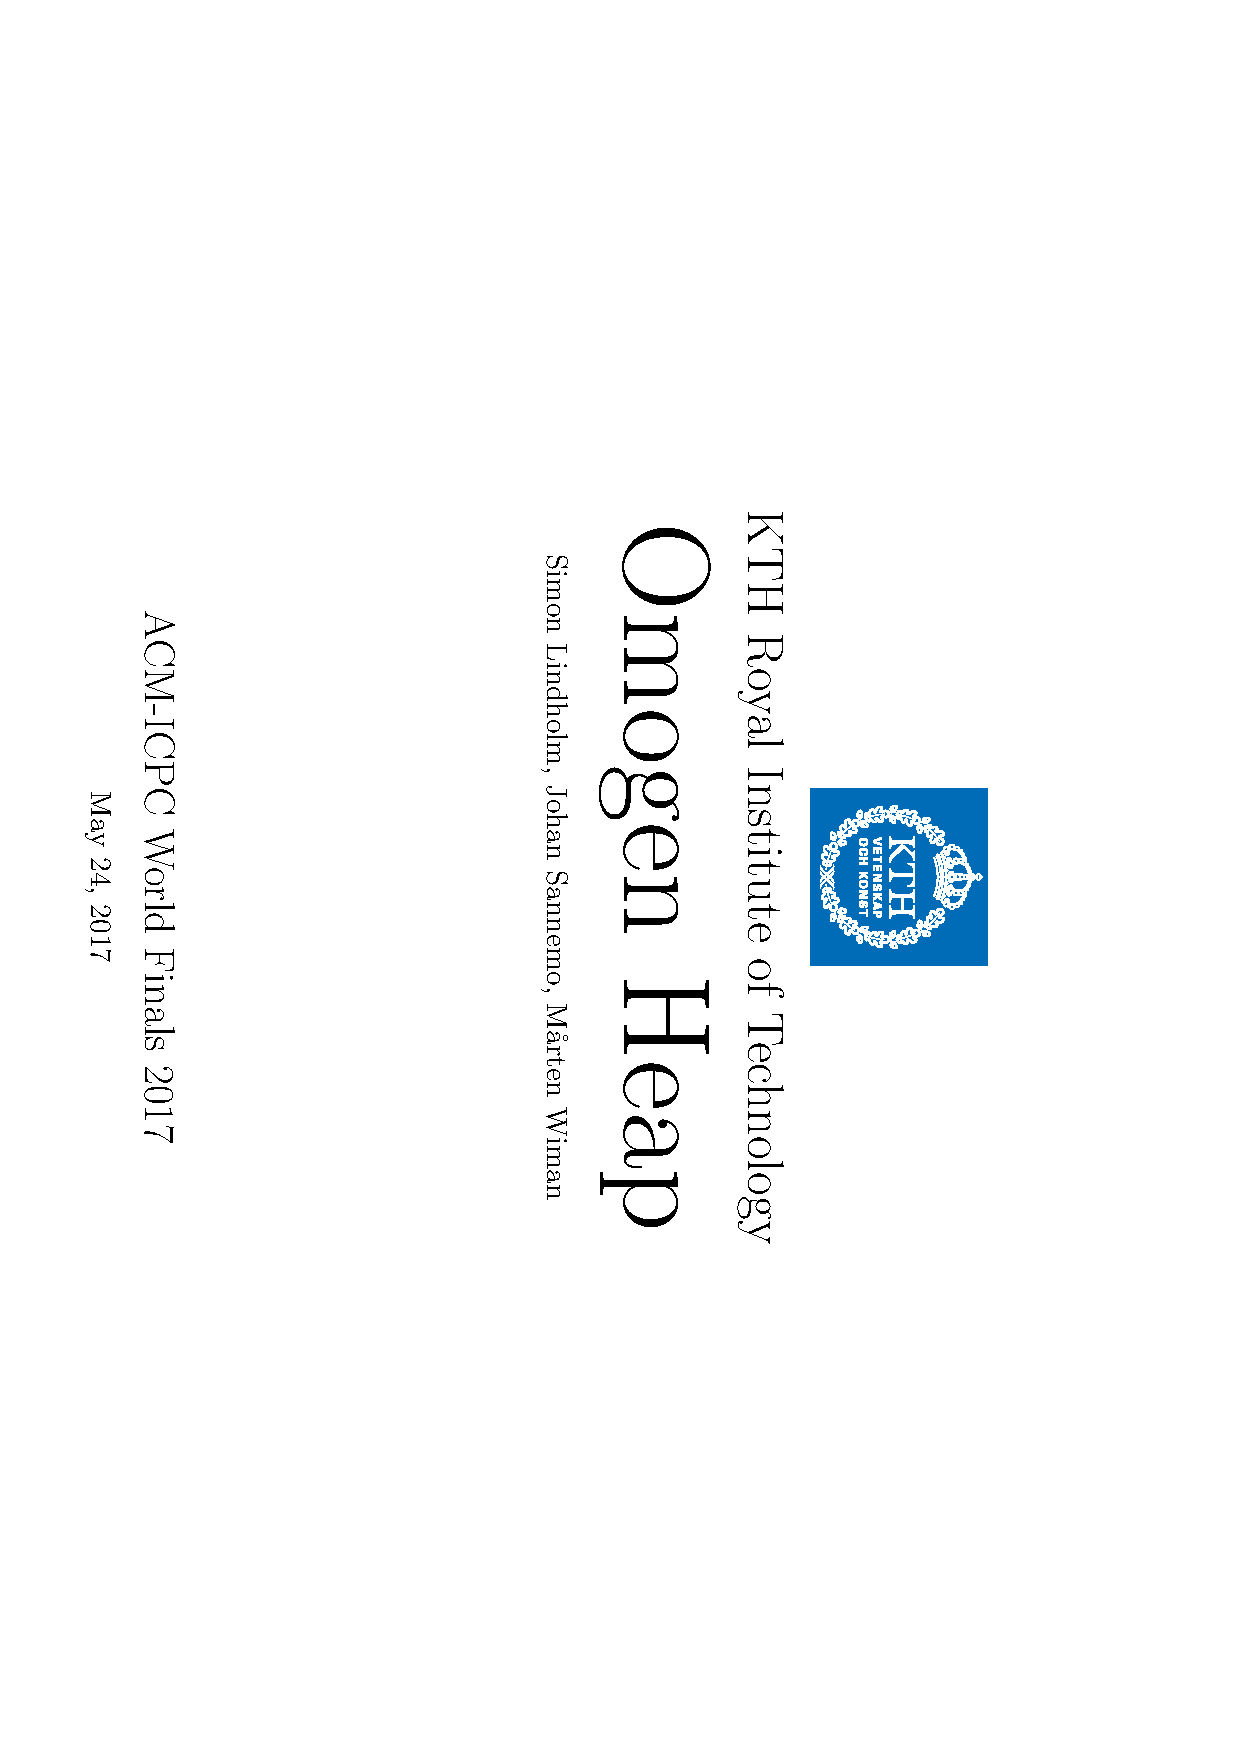
\includepdf[page={2-26},landscape = true,noautoscale = true,delta = 2cm 2cm,scale = 0.9]{kactl_90.pdf}
\end{document}
